% Chapter 3

\chapter{Instrumentation: Fast Temperature Program GC} % Write in your own chapter title
\label{Chapter3}
\lhead{Chapter 3. \emph{Fast GC}} % Write in your own chapter title to set the page header

\section{The nature of the problem}

Before we look at the experimental work, it would be useful to put the research problem into the context of problems in general. I will be using Ulrich's \cite{Ulrich2011} taxonomy. (Figure~\ref{fig:ProblemTaxonomy})

\begin{figure}[htbp]
	\centering
	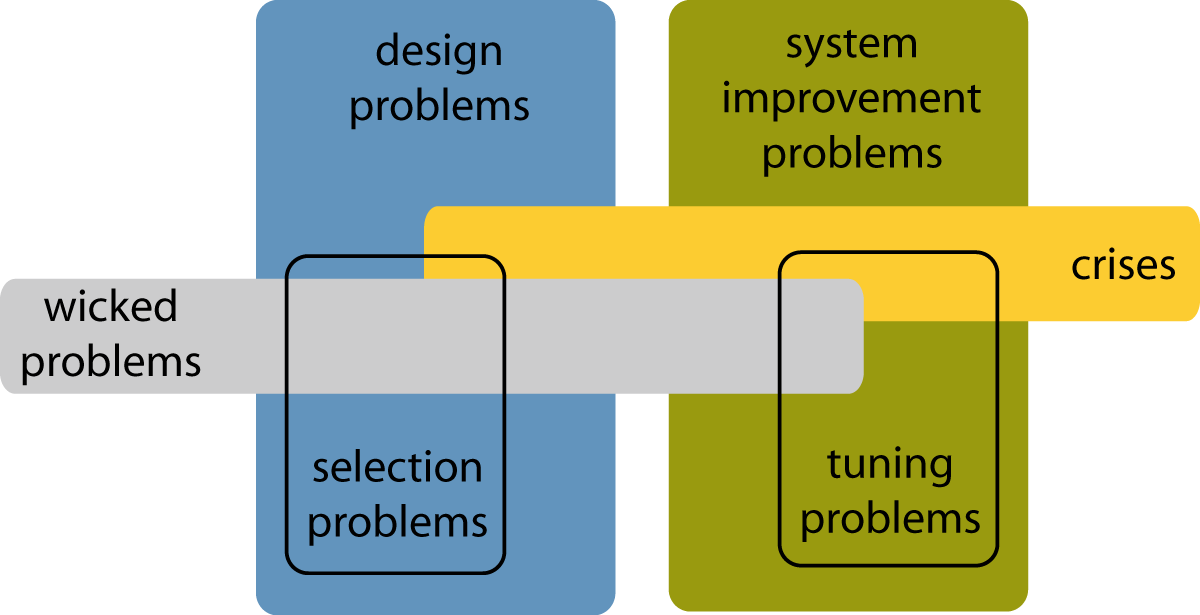
\includegraphics[width=0.8\textwidth,natwidth=4.17in,natheight=3.32in]{./Figures/ProblemTaxonomy}
	\rule{35em}{0.5pt}
	\caption[Taxonomy of Problems]{A simple taxonomy of problems}
	\label{fig:ProblemTaxonomy}
\end{figure}

Not every research problem will, in the end, contain a design problem. In terms of analytical chemistry, say a system improvement problem such as needing to improve resolution between critical peaks, may easily be solved by simply optimizing the chromatography, making it a tuning problem. But it might also be that the system improvement (increasing resolution) will demand a new stationary phase. This then becomes a selection problem, a subste of design problems. 

Many chromatographic problems are system improvement problems, or selection problem. Method development in GC is typically a selection problem: select stationary phase, select flow rates and temperature programmes. Often the design problems of analytical chemistry lies in sampling and sample preparation

In developing our system, we were faced by a true design problem, in at least three dimensions: mechanical, software/electronics, and chromatographic. 

\section{Why fast temperature program gas chromatography?}

The use of temperature programming for GC in \SFCxGC is required by the wide range of boiling points expected in the second dimension. Otherwise the general elution problem will cause the spreading out of peaks of high-boiling compounds, or the loss of resolution of low-boiling peaks, depending on the temperature 

Fast temperature programming is desirable because of the expected duration of the \SFCxGC run. 

$t_{total} = t_{SFC total} + \frac{t_{SFC total}}{t_{SFC fraction}} \times t_{GC run}$

If a typical SFC run takes 20 minutes, and fractions are collected for every 5 seconds of SFC run, it means there will be 20*60/5 = 240 fractions collected. Each of these must become a GC run. If each GC run took a minute, the \SFCxGC run would last 4 hours. This is not unheard of in chromatography, but \GCxGC runs take as long as the first dimension run, so \SFCxGC would not compete in terms of time

Obviously the $t_{SFC fraction}$ can be increased for a smaller $t_{total}$ but too large an SFC fraction can overload the GC column.

\section{Fast GC theory}

A specific separation problem needs a certain number of theoretical plates, $N_{req}$. In fast chromatography the question is how this number of plates can be achieved in the shortest time. 

\begin{equation}
t_r = (1+k) N_{req}^\frac{3}{2}\frac{9}{8}\sqrt{3}F(k)\left[\frac{\eta}{p_0 D_{m,o}}\right]^\frac{1}{2}d_cS2T
\label{eqn:tr}
\end{equation}

For a a

\begin{equation} 
N_{req}= 16R^2_s\left[\frac{1+k}{k}\right]^2\left[\frac{\alpha}{\alpha-1}\right]^2
\label{eqn:Nreq}
\end{equation}

\begin{equation}
F(k) = frac{1+6k+11k^2}{96(1+k)^2}
\label{eqn:EquationLabel}
\end{equation}

\begin{figure}[htbp]
	\centering
	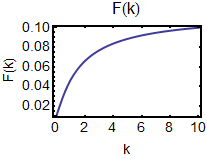
\includegraphics[width=0.8\textwidth,natwidth=4.17in,natheight=3.32in]{./Figures/F(k).png}
	\rule{35em}{0.5pt}
	\caption[Dependence of F on k]{Dependence of F on k}
	\label{fig:F(k)}
\end{figure}

Figure~\ref{fig:F(k)} shows the dependence of $F$ on $k$. This shows that lower k gives smaller F. This is in keeping with the $(1+k)$ term, so that there is no minimum $t_r$ dictated by $k$.

Examining Equation~\ref{eqn:tr} it becomes apparent that to minimize $t_r$ one can reduce $N_{req}$ or the last two terms. 

$N_req$ can be reduced by minimizing the resolution to the lowest sufficient value. This means leaving some peaks unresolved. 

Reducing the resolution can be achieved by: 
\begin{itemize}
	\item using a shorter column
	\item using a higher gas flow 
	\item using a higher temperature
	\item using temperature programming
	\item using pressure or flow programming
	\item using a thinner film
\end{itemize}

Improving the selectivity ($\alpha$) will also reduce the number of plates needed. This can be improved by:
\begin{itemize}
	\item selecting a different stationary phase
	\item using selective detection, for example an electron capture detector.
	\item using MS detection.
\end{itemize}


Further

%The Van Deemter curve predicts the optimum HETP. There is no way of improving the resolution. In general, doing faster GC, using shorter columns and increasing the mobile phase flow will lead to poorer resolution. However, if the peak density can be reduced, there might be surplus resolution, and the speed of the separation can be improved. The surplus resolution can be generated either on the detector side, or on the sample side.

%On the detector side, surplus resoluton can be generated by selective detection, such as 

%On the sample side, surplus resolution can be 



\section{How the temperature measurement works}

Consider two resistors in series $R_{col}$ and $R_{ref}$, with $R_{col} \gg R_{ref}$. $R_{col}$ represents the resistance of the column, and $R_{ref}$ represents the resistance of the reference column. Because of the resistance ratio most of the heat developed in the circuit is developed in $R_{col}$. 

The circuit is supplied by a voltage $V_{sup}$, in general an unknown value. $V_{col}$ and $V_{ref}$ represents the voltage drop over the respective resistors. 

Because the current $I$ through the circuit is the same for both $R_{col}$ and $R_{ref}$, it is true that $\frac{R_{col}}{V_{col}}=\frac{R_{ref}}{V_{ref}}$, and therefore \begin{equation}R_{col} = R_{ref}\frac{V_{col}}{V_{ref}} \end{equation}

The voltage drop across $V_{ref}$ is small, and therefore it is amplified by the amplifier with gain $g$, so that $V_b = gV_{ref}$

$V_{sup} = V_{col} + V_{ref}$ 

$V_{sup}=dV + V_b$

$V_{col} + V_{ref} = dV + V_b$

$V_{col} + V_{ref} = dV + gV_{ref}$

$V_{col} = dV + gV_{ref} - V_{ref} $

$V_{col} = dV + V_{ref}(g - 1)$

$\frac{\displaystyle V_{col}}{\displaystyle gV_{ref}} = dV/gV_{ref} + V_{ref}(g-1)/gV_{ref}$

$\frac{\displaystyle V_{col}}{\displaystyle V_{ref}} = gdV/gV_{ref} + gV_{ref}(g-1)/gV_{ref}$

$\frac{\displaystyle V_{col}}{\displaystyle V_{ref}} = gdV/V_b + (g-1)$

This proves that $\frac{\displaystyle V_{col}}{\displaystyle V_{ref}}$ is a linear function of $dV/V_b$. A quick check for correctness of the expression: for a unity-gain amplifier $g = 1$, and $\frac{\displaystyle V_{col}}{\displaystyle V_{ref}} = dV/V_b$.


\subsection{Assumptions}

The assumption is that the temperature is a function of the resistance of the column, or $T = f(R_{col})$. Because $R_{col}=m(^{dV}/_{V_b}) + c$, we can say that $T = f'(^{dV}/_{V_b})$. Through a calibration procedure $f'$ can be approximated by a polynomial. 

\section{Calibrating the Column}

The calibration of coaxial heater. 

\subsection{Thermocouple}

The problems of measuring a temperature inside a tube with a bore of 1 mm is not trivial.

The following methods can be used to measure temperatures.
\begin{itemize}
	\item Liquid-in-glass thermometers
	\item Sealed liquid or gas sensing instruments and bimetallic sensors.
	\item Electrical Resistance Temperature measurement using metallic sensors
	\item Thermistors and semiconductors
	\item Thermoelectric temperature measurement
	\item Disappearing filament optical pyrometer
	\item Photoelectrical optical pyrometers
	\item Total radiation pyrometers.
\end{itemize}

Liquid-in-glass thermometry would not be applicable because of the size of the devices, and because they don't give a desirable electrical signal. Radiant energy methods would not be of much use at the lower end of the temperature range, and will also only measure the outside wall surface temperature of the heater. This leaves us with resistance temperature measurement with metallic sensors, thermistors and semiconductors, and thermoelectric.

Thermistor and semiconductor devices could, in principle be made small enough for the job, but affordable packages are too large. Besides that, the operating temperature range is a bit extreme for semiconductors that generally have an upper temperature limit of about 200 (?) �C. 

Electrical resistance measurement using metallic sensors are quite feasible, if a sensing element of the right dimensions are available. These are not easy to find. Additionally, because long thin wires would be needed to connect the sensing element to the electronics.

Thermoelectric temperature measurement then remains. This uses the effect that a circuit of two dissimilar metals will generate a voltage when there is a temperature gradient along the conductors. The voltage generated is a function of the temperature difference between the junctions of the two metals. Thermocouples are widely used in industry for measuring temperatures, and the technology is well established. Thermocouple wire can be purchased in varying gauges, down to 25 $\mu$ m in diameter. 

McGee \citep{Mcgee1988} states that thermocouple junctions can be made by welding, crimping, soft soldering, hard soldering, bolting, or simply twisting the wires together.

Because of the temperature range expected to be measured (-50�C to 350�C) the option of soft soldering does not apply. Because of the possibility of corrosion, bolting or twisting the wires together are not good options.

This leaves welding, crimping and hard soldering. The option of crimping was not explored, chiefly because the author has no knowledge of the technology or of any devices that could do this. Two patents (ref?) (ref?) available on the topic shows another problem: the final crimped connection has a diameter many times the diameter of the wire. This precludes the application of crimping in this context.

How the thermocouple probe was made:

\begin{enumerate}
	\item A piece of 0.25 mm polyimide-coated fused-silica capillary of about 500 mm length was cut and mounted with sticky tape on a wooden metre stick.
	\item A longer length of 0.1 mm fused-silica capillary was threaded through the 0.25 mm capillary.
	\item The end of one of the thermocouple wires was inserted into the end of the 0.1 mm capillary. A drop of cyanoacrylate adhesive was touched to the end of the capillary. Capillary action drew the liquid adhesive into the capillary and fixed the wire in place.
	\item The wire was drawn carefully into the capillary by pulling on the 0.1 mm capillary.
	\item Once the end of the wire protruded through the end of the 0.25 mm capillary the end of the 0.1 mm capillary was cut off.
	\item The wire was anchored at one end with adhesive tape, pulled tight, and anchored at the other end. 
	\item The procedure was repeated for the other wire.
	\item The two thermocouple wires (Goodfellow) was clamped in a twisting bar. The twister bar has a square profile, 8 mm on a side.
	\item The wires were flamed with a cigar lighter until they were red a dull red hot. (At any higher temperature the wires would melt.) This chars the polyimide coating.
	\item The flamed portion of the wires were lightly sanded with 1200 grit water paper. A pair of small pliers had its beak lined with the abrasive, and lightly stroked up and down the wire to remove the char.
	\item A 6 mm tube was inserted between the wires to serve as spacer. and moved until about 10mm away from the twister bar.
	\item The wires were twisted by turning the twister bar until the twister portion was about 5mm long.
	\item The spools were rewound to retract the wire, until the start of the twist rested on the clamping bar.
	\item The clamping weight was lowered onto the clamping bar, keeping the pair or wires in place.
	\item A small pair of scissors was used to snip off the end of the
	\item The welding electrode was brought into position. This was a carbon rod in the form of a pencil lead (Schwann Stabilo), 2 mm in diameter, mounted on a screwing connector. The welding circuit consisted of a bench power supply set to approximately 20V. connected. The negative terminal was clamped to the aluminium base plate of the microscope, on which rested the brass clamp bar. The positive terminal was clamped to the carbon electrode. A voltage of approximately 23 V was applied.
	\item It was discovered that the carbon electrode should not have a polished end, but a roughly broken end. 
	\item The electrode was moved closer to the clamped twisted wire.
	\item At the right point a spark would jump from the carbon to the wire, melting the end of the wire. The molten wire would draw into a globule on the end of the wire, withdrawing from the electrode and so breaking the spark, ending the heating.
	\item If the wire would actually touch the electrode the wire would heat up red hot and melt off, usually destroying the twist and requiring making a new twist.
	\item If all went well, there would be a hemispherical weld at the end of the twist where the two wires would be joined.
	\item The thermocouple wires was withdrawn into the capillary until the end just protruded, kept in place with a pair of rubber-tipped self-closing tweezers.
	\item If two sets of thermocouples were needed, the procedure would be repeated for another pair of wires.
	\item The wires would be pulled back, one pair at a time.
	\item The other end of the capillary was taped to the connector pad.
	\item The wires was flamed and scraped to remove the polyimide isolation, and screwed down on a screw connector block.
	\item The resistance between the protruding end of the thermocouple and the connector block was measured to ensure electrical connection. The resistance for the Chromel is 1440 $\Omega{m}^{-1}$, and for the Alumel 600 $\Omega{m}^{-1}$
\end{enumerate}

\section{Thermocouple Welding}

\begin{figure}[htbp]
	\centering
	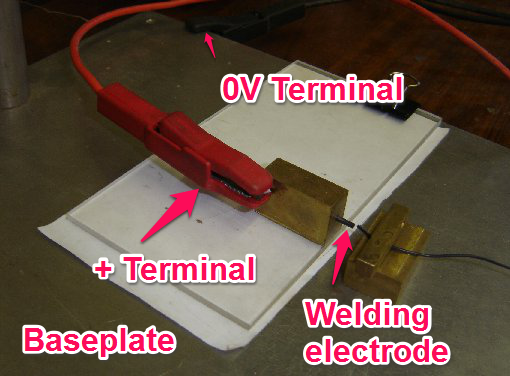
\includegraphics[width=0.8\textwidth,natwidth=4.17in,natheight=3.32in]{./Figures/Welder.png}
	\rule{35em}{0.5pt}
	\caption[Fine-wire welder]{A view of the fine-wire thermocouple welder.}
	\label{fig:Welder}
\end{figure}

\begin{figure}[htbp]
	\centering
	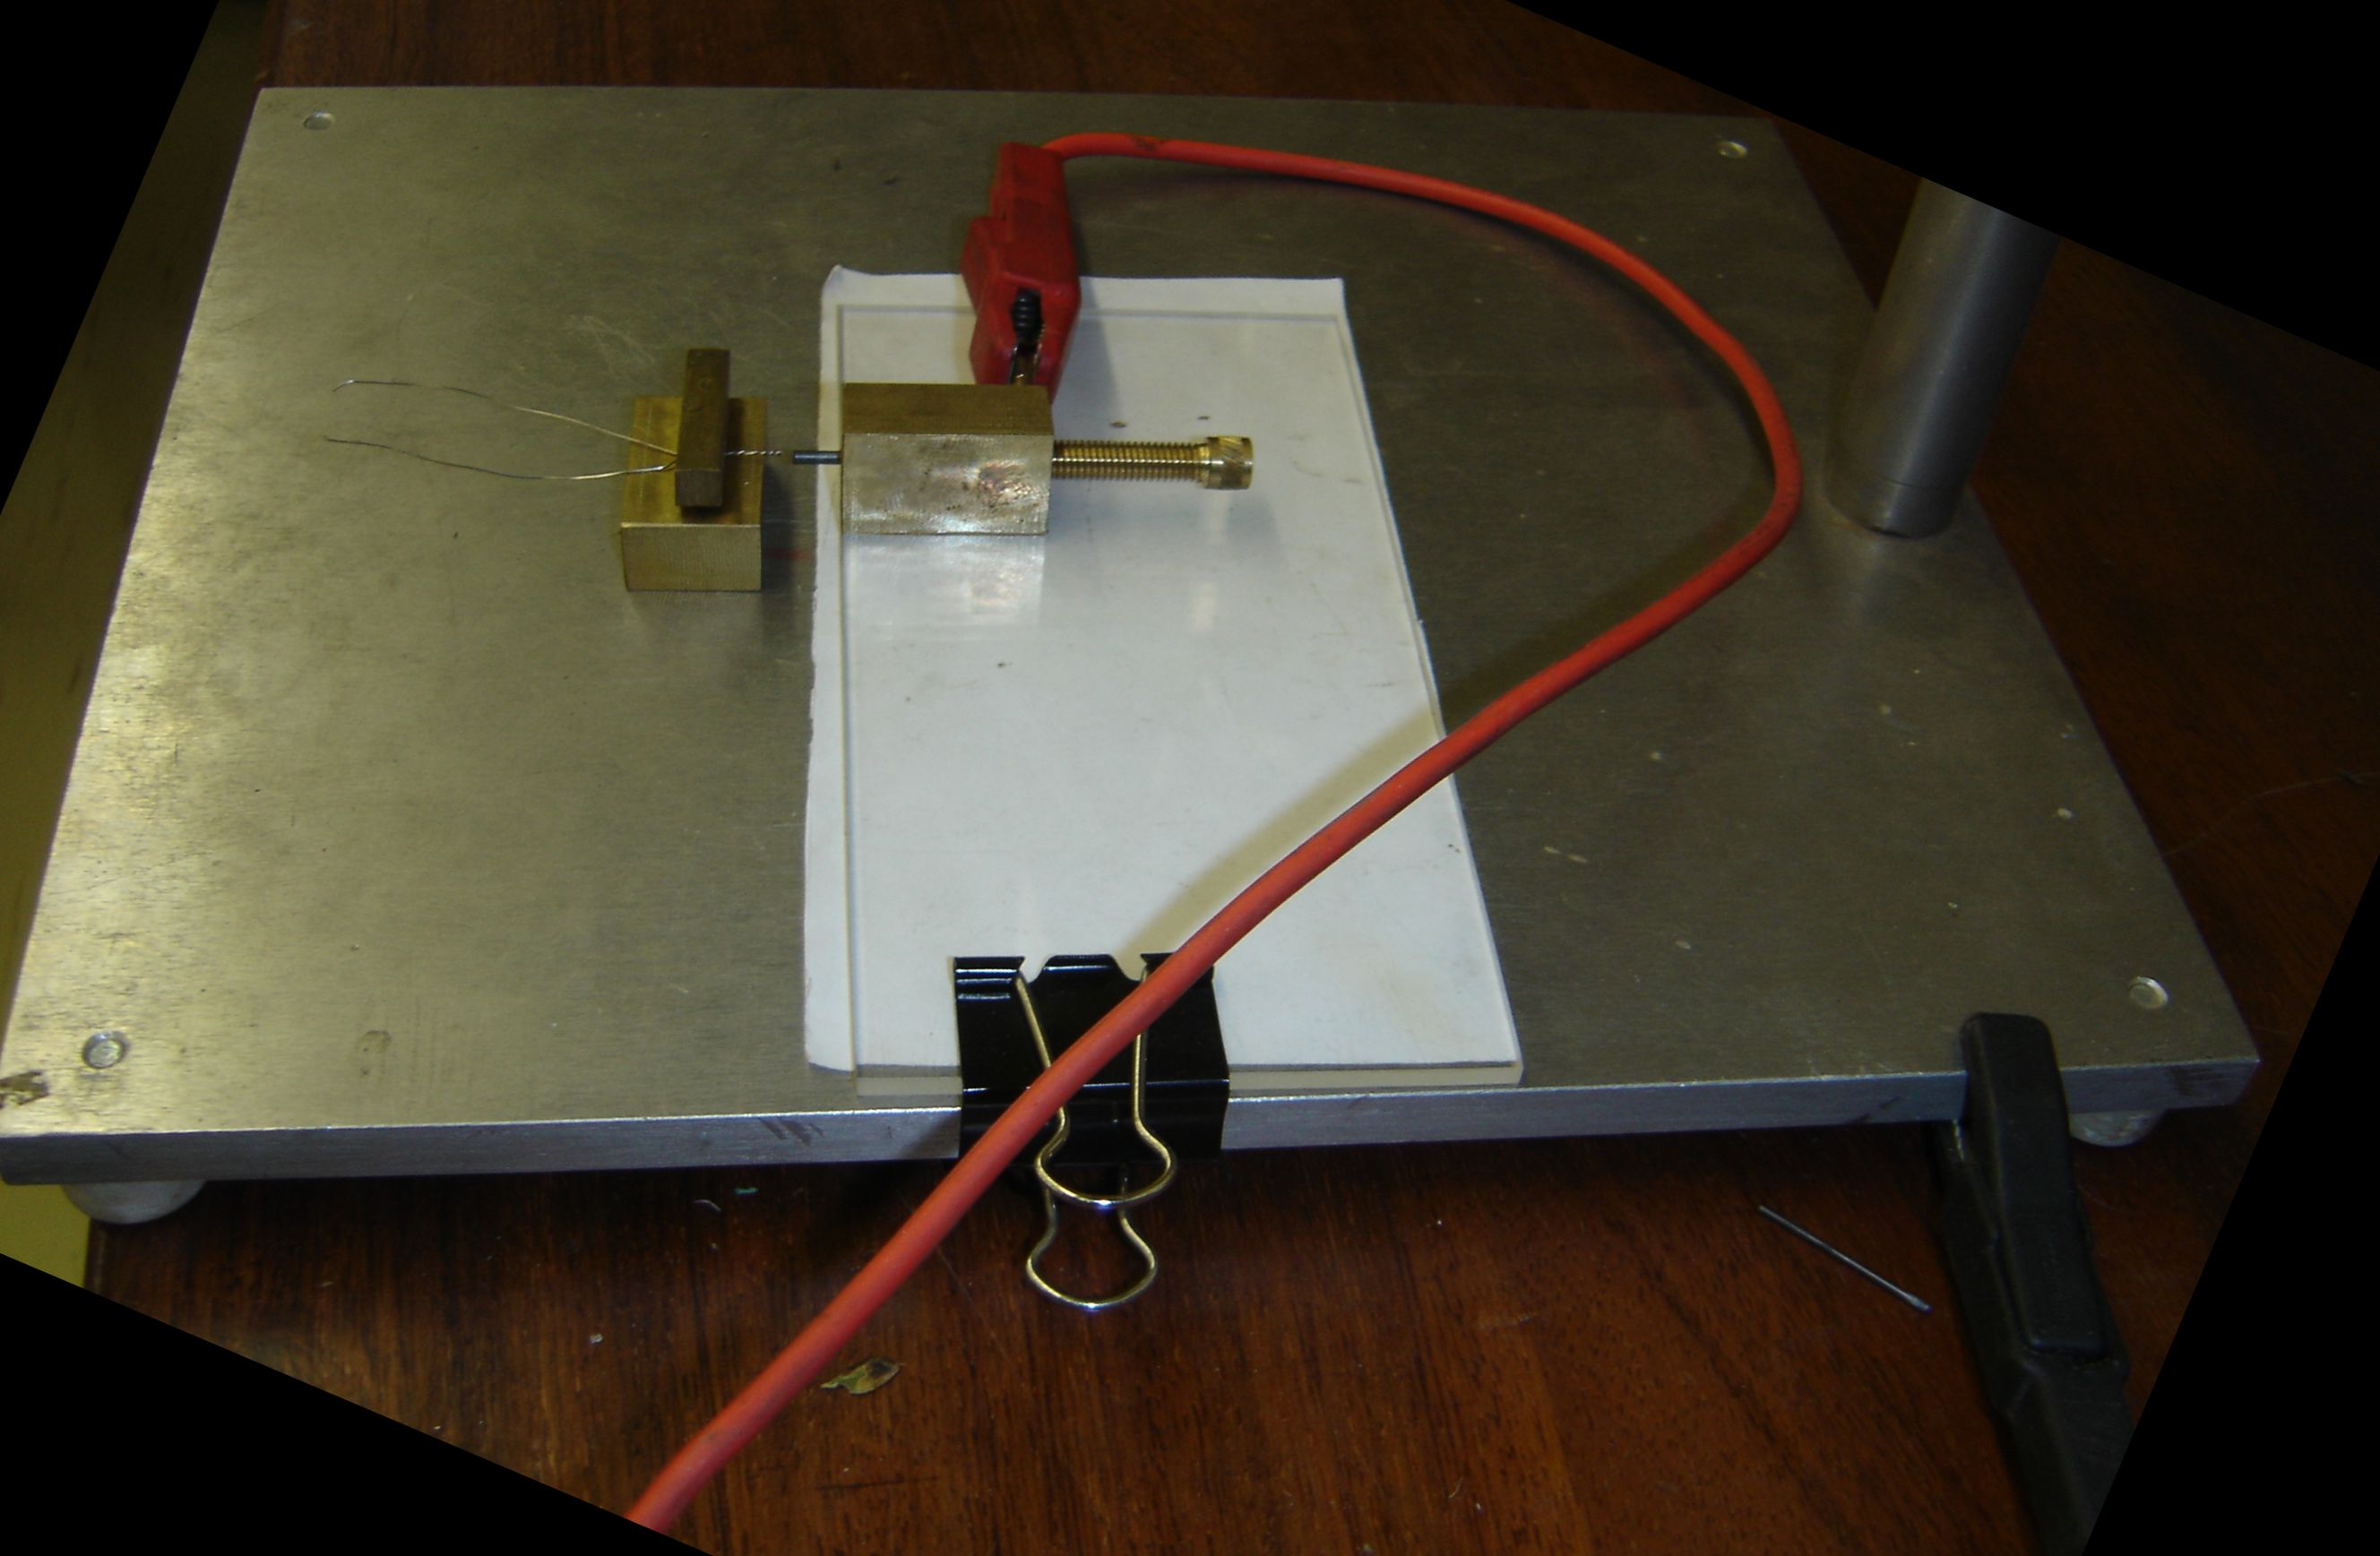
\includegraphics[width=0.8\textwidth,natwidth=4.17in,natheight=3.32in]{./Figures/Welder2.jpg}
	\rule{35em}{0.5pt}
	\caption[Fine-wire welder]{A view of the fine-wire thermocouple welder. The wire shown is much thicker than that actually used. It is shown clamped between the clamping bar and the clamping weight. A thin sheet of Perspex serves to isolate the positive electrode from the negative base. The carbon electrode can be advanced towards the thermocouple twist using the screw. The black clamp at the bottom right-hand corner attached to the base plate and the red clamp attached to the screw housing provide a potential difference of approximately 20 V between the carbon electrode and the thermocouple.}
	\label{fig:Welder2}
\end{figure}


\begin{figure}[htbp]
	\centering
	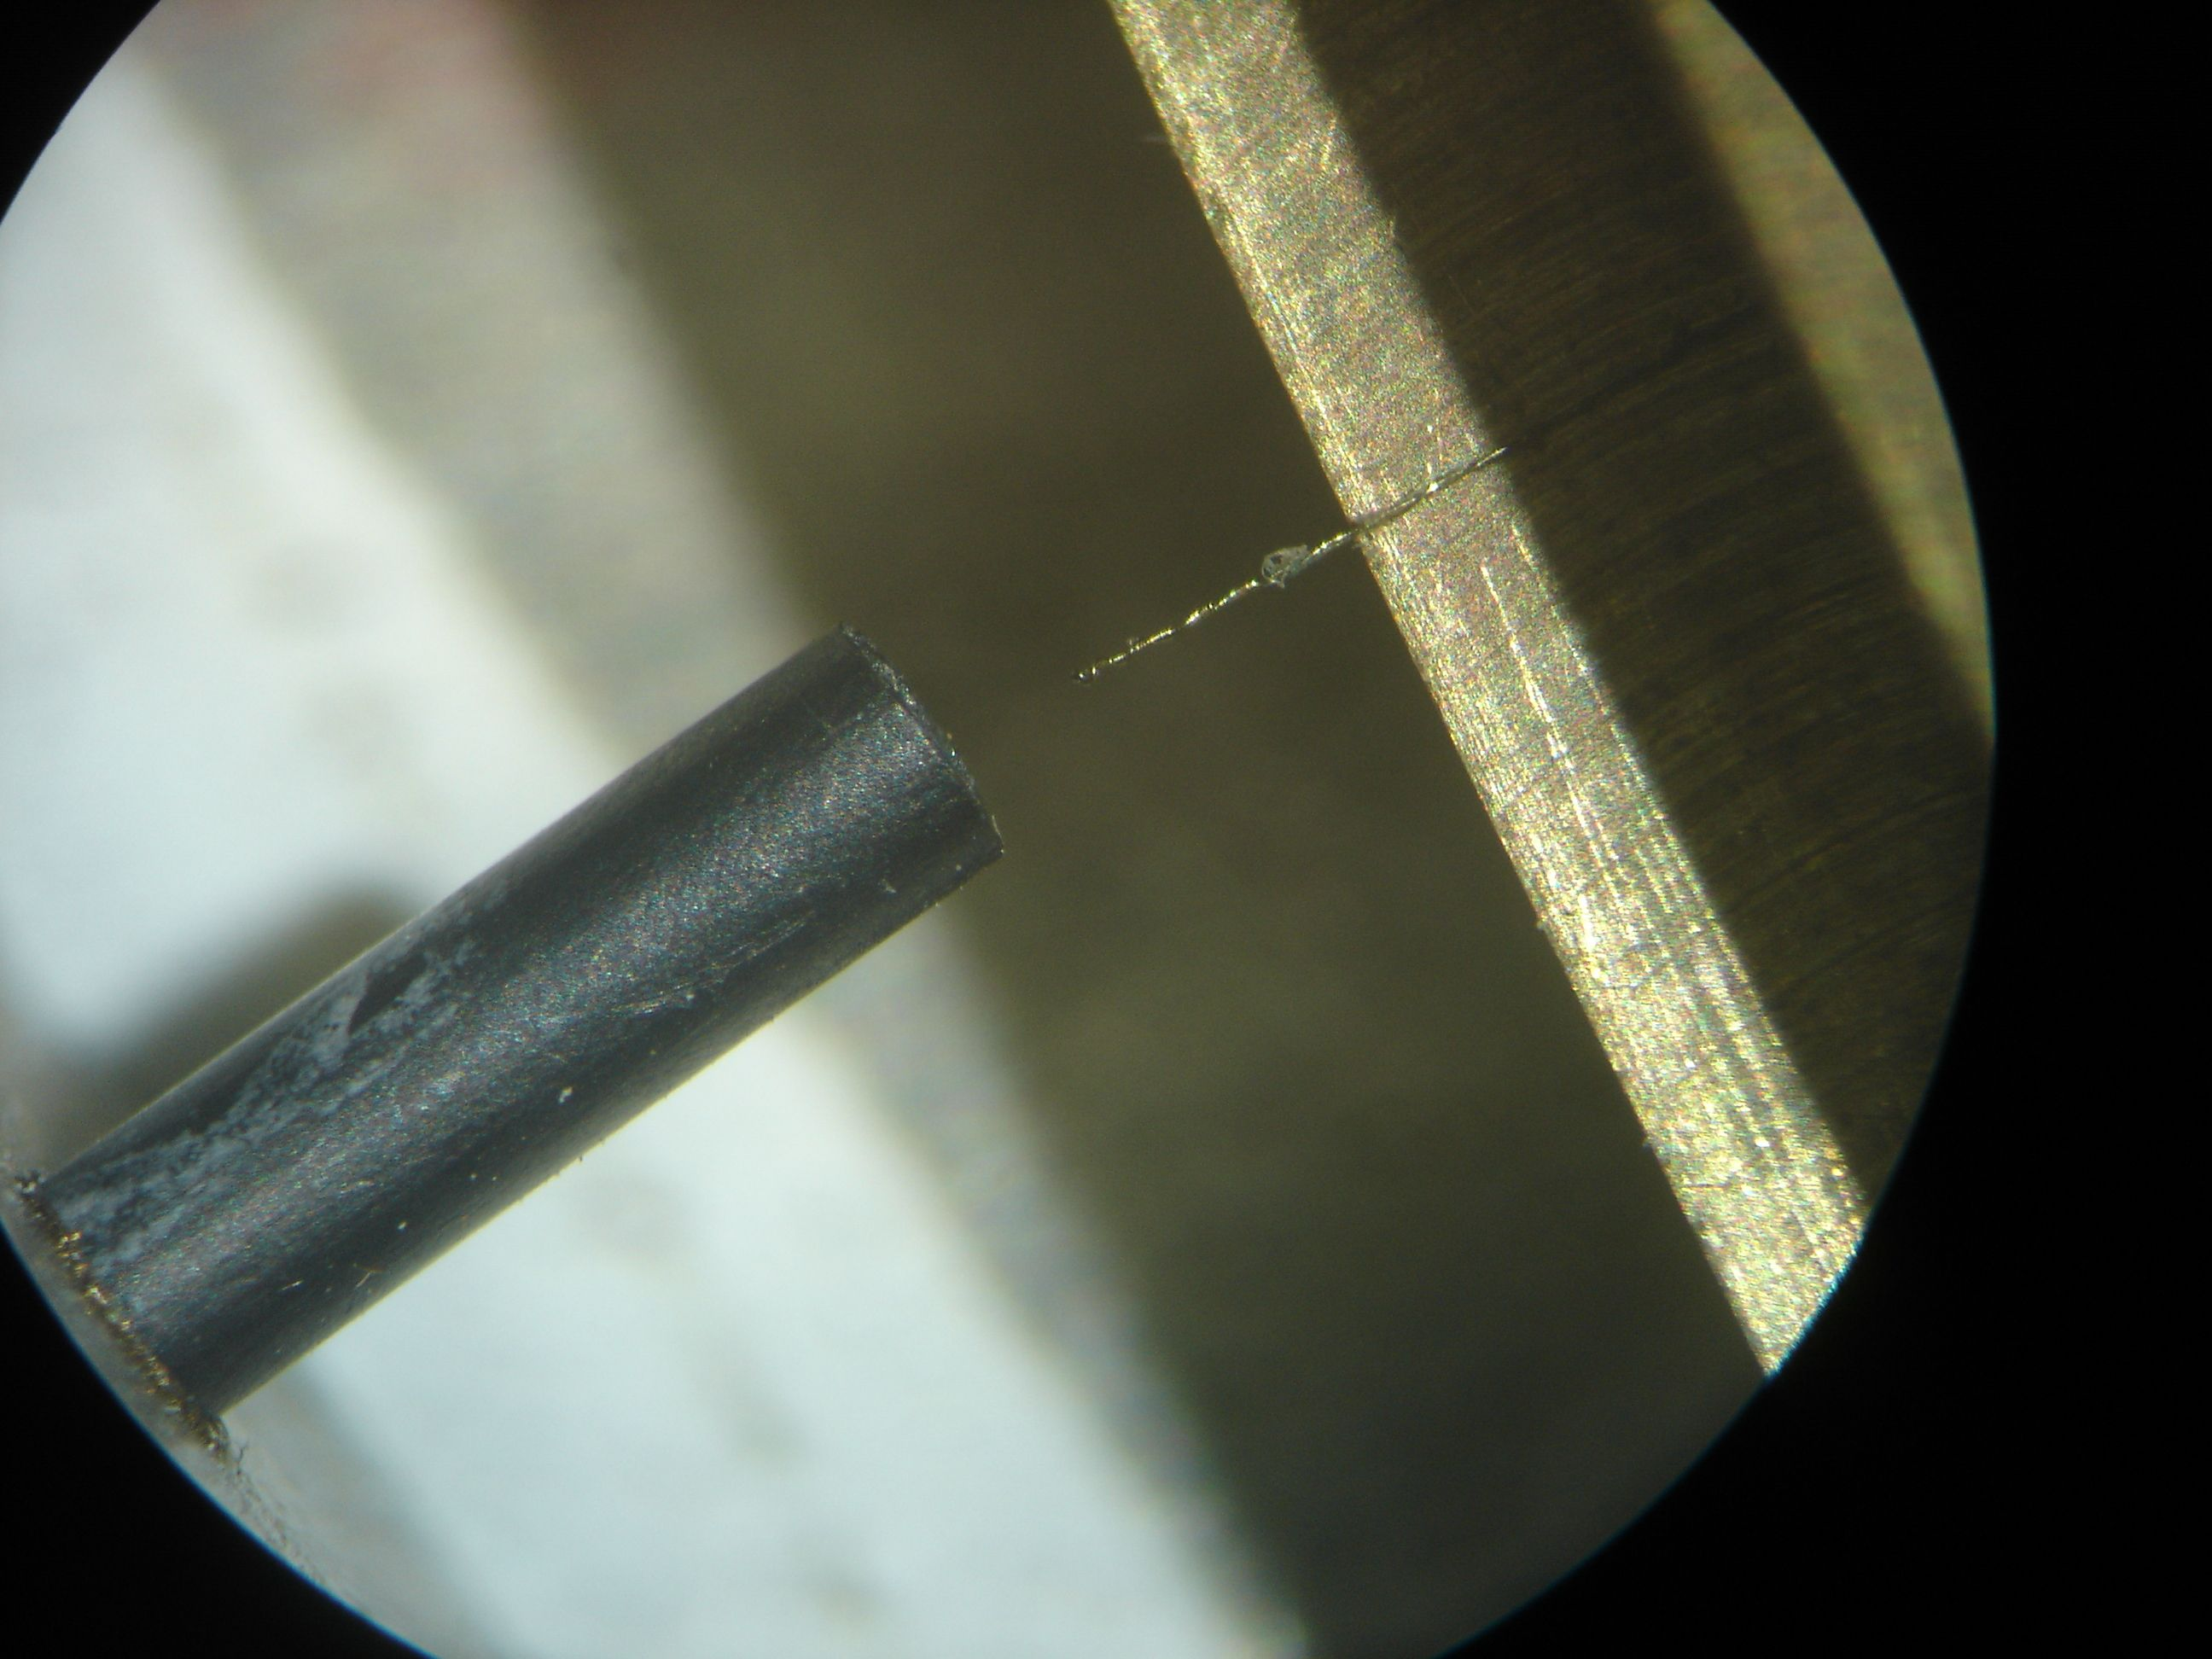
\includegraphics[width=0.8\textwidth,natwidth=4.17in,natheight=3.32in]{./Figures/WelderMicro.jpg}
	\rule{35em}{0.5pt}
	\caption[A microphoto of a thermocouple twist ready to be welded.]{A microphoto of a twisted wire ready to be welded. The black carbon electrode is 2mm in diameter.}
	\label{fig:TheFigureLabel}
\end{figure}


\section{Extra}